\documentclass[12pt]{article}
   
\usepackage[utf8]{inputenc}
   \usepackage{graphicx}
   \usepackage{float}
   \usepackage{subcaption}
   %\usepackage{mathtools}
   \usepackage{amsmath}
   
   \addtolength{\hoffset}{-0.7in}
   \addtolength{\textheight}{1.5in}
   \addtolength{\textwidth}{1.5in}
   \addtolength{\voffset}{-1in}
%
% Title.
\title{EE230: Experiment 4\\
Precision Rectifiers}

% Author
\author{Hitesh Kandala, 180070023}

% begin the document.
\begin{document}

% make a title page.
\maketitle

\section{Overview of the experiment}

\subsection{Aim of the experiment}
The goal of this experiment is to analyse/understand the working of different types of rectifiers which are based on the Op-amp and the Diode interconnections and their behaviour at low and high input signal frequencies.

% \begin{itemize}
%     \item Wire up the circuit of half-wave precision rectifier and verify the half-wave rectification.
%     \item Wire up the circuit of improved half-wave precision rectifier-A and verify the half-wave rectification.
%     \item Wire up the circuit of improved half-wave precision rectifier-B and verify the half-wave rectification.
%     \item Wire up the circuit of full-wave precision rectifier and verify the full-wave rectification.
% \end{itemize}

% \subsection{Theory} 
       
\section{Experimental results}

\subsection{Simple half-wave rectifier}
        \begin{figure}[H]
            \centering
            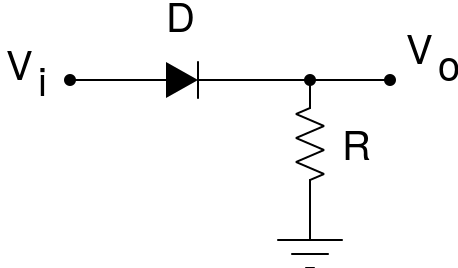
\includegraphics[width = 0.5\linewidth, height = 2in]{reports/lab3/half.png}
            \caption{Half-wave rectifier}
        \end{figure}
        \\
        This is a simple half-wave rectifier with 
        \begin{equation}
         V_o = V_i - V_{ON}   
        \end{equation}
    
        \begin{figure}[H]
            \centering
            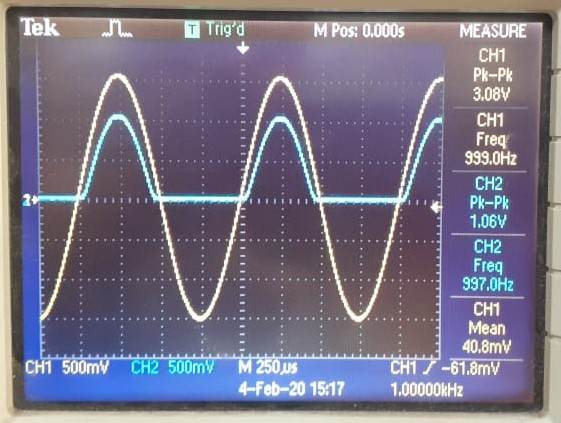
\includegraphics[width = 0.6\linewidth, height = 2.8in]{reports/lab3/vdon-waveform.jpeg}
            \caption{Waveform of simple Half-wave rectifier}
        \end{figure}
        \\
        From fig. 6, we get $V_o = 1.06 V$ peak for $V_i = 1.54 V$ peak.
        \begin{equation}
           \boxed{V_{ON} = 0.48V}   
        \end{equation}
        \\
        Following is the $V_o$ vs $V_i$ plot, the curve follows equation 1.
        \begin{figure}[H]
            \centering
            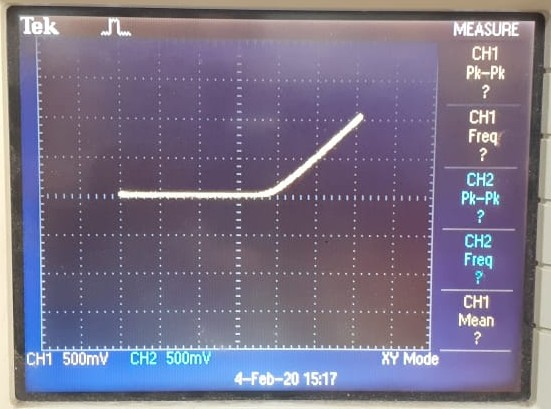
\includegraphics[width = 0.6\linewidth, height = 2.5in]{reports/lab3/vdon.jpeg}
            \caption{$V_o$ vs $V_i$ relationship}
        \end{figure}
        \\
        From figure 3, we can see that the value of $V_{ON}$ lies between 0.4V to 0.5V
        
\subsection{Half-wave precision rectifier}
        \begin{figure}[H]
            \centering
            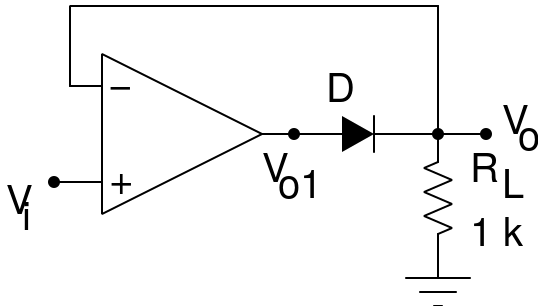
\includegraphics[width = 0.6\linewidth, height = 2in]{reports/lab3/half-rect.png}
            \caption{Half-wave precision rectifier}
        \end{figure}
        
      \\
         The actual value of resistance $R_L$ is $0.96k\Omega$
        \\
        
      \textbf{(A) With $\mathbf{f = 100Hz :}$}\\
         
        The observed waveform of this rectifier is: 
        \begin{figure}[H]
            \centering
            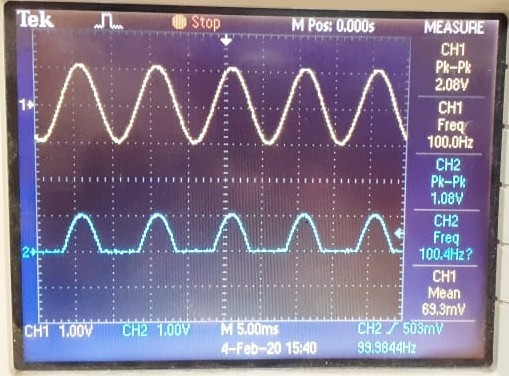
\includegraphics[width = 0.5\linewidth, height = 2.5in]{reports/lab3/half-wave-2.jpeg}
            \caption{Waveform of Half-wave precision rectifier}
        \end{figure}
        \\
        $V_o$ vs $V_i$ relationship comes out to be linear for $V_i > 0$, passing through origin.
        \begin{figure}[H]
            \centering
            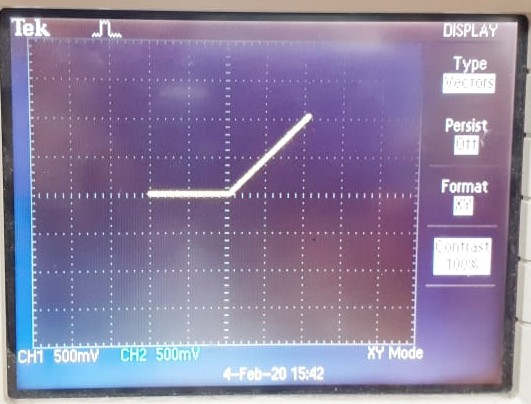
\includegraphics[width = 0.6\linewidth, height = 2.5in]{reports/lab3/half-wave-xy.jpeg}
            \caption{$V_o$ vs $V_i$ relationship}
        \end{figure}
        \\
        
        \textbf{(B) With $\mathbf{f = 5kHz :}$}\\
    
        The observed waveform of this rectifier is: 
        \begin{figure}[H]
            \centering
            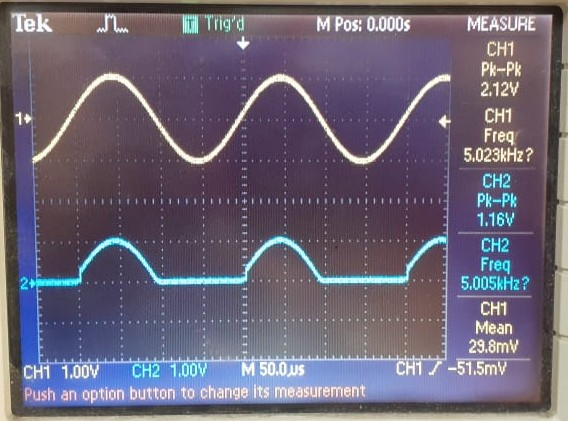
\includegraphics[width = 0.6\linewidth, height = 2.5in]{reports/lab3/half-wave-5khz.jpeg}
            \caption{Waveform of Half-wave precision rectifier}
        \end{figure}\\
        \\
        The op-amp goes into saturation for $V_i < 0$. Now as $V_i > 0$, the op-amp has to come out of saturation and $V_{o1}$ has to go from $-V_{sat}$ to some V in the linear region. Now, this process is relatively slow and it is limited by the op-amp slew rate and therefore we cannot operate the circuit at higher frequencies. We can look at the above waveform to see that there is distortion in waveform as $V_i$ becomes positive.
        \\
        
\subsection{Improved half-wave precision rectifier-A}
      \begin{figure}[H]
            \centering
            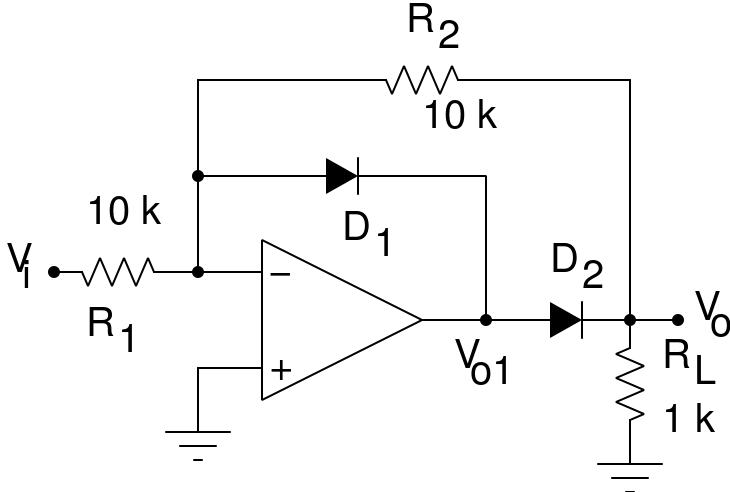
\includegraphics[width = 0.5\linewidth, height = 2.5in]{reports/lab3/half-rect-A.png}
            \caption{Improved half-wave rectifier-A}
        \end{figure}
        \\
        The actual resistance of resistors shown in fig 8 are,
        $R_1 = 9.77\Omegak$, $R_2 = 9.66k\Omega$, $R_L = 0.96k\Omega$.\\
        In this rectifier, the current will flow for $V_i < 0$.
        \\
        
        \textbf{(A) f = 100Hz}\\
        
        The observed waveform of this rectifier is: 
        \begin{figure}[H]
            \centering
            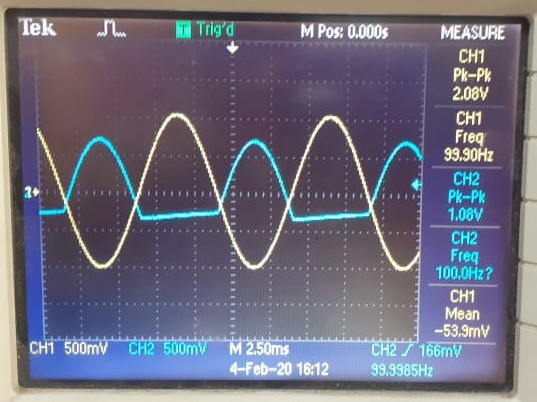
\includegraphics[width = 0.5\linewidth, height = 2in]{reports/lab3/half-wave-rect-A-100k.jpeg}
            \caption{Waveform of Improved half-wave rectifier-A}
        \end{figure}
        \\
        $V_o$ vs $V_i$ relationship is given by
        \begin{equation}
            V_o = -\frac{R_2}{R_1}\times V_i
        \end{equation}
        \begin{figure}[H]
            \centering
            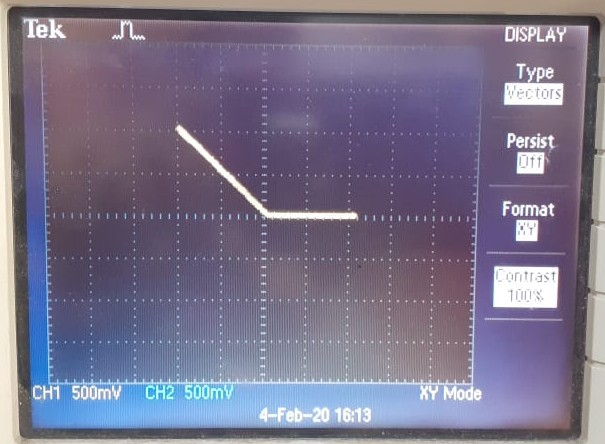
\includegraphics[width = 0.6\linewidth, height = 2.5in]{reports/lab3/half-wave-rect-A.jpeg}
            \caption{$V_o$ vs $V_i$ relationship}
        \end{figure}
        \\
        
        \textbf{(B) With $\mathbf{f = 5kHz :}$}\\
    
        The observed waveform of this rectifier is: 
        \begin{figure}[H]
            \centering
            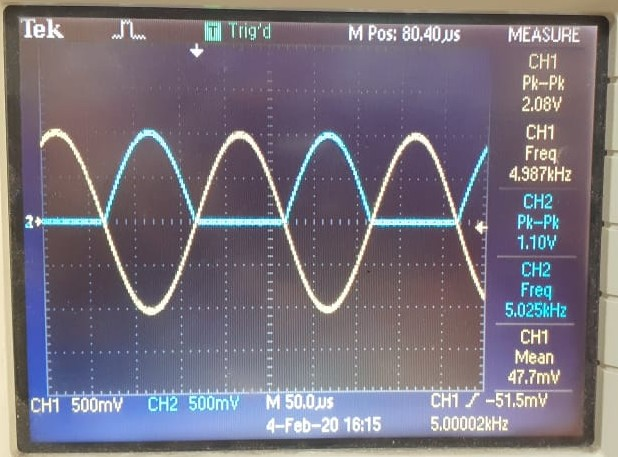
\includegraphics[width = 0.6\linewidth, height = 2.5in]{reports/lab3/half-wave-rect-A-5k.jpeg}
            \caption{Waveform of Improved half-wave rectifier-A}
        \end{figure}
        \\
        Here the rectifier conducts for $V_i < 0$. For $V_i > 0$, $V_o$ goes to 0 because at this point the diode D1 conducts and completes the feedback loop not allowing the op-amp to go in saturation. Therefore distortion in the waveform is absent for higher frequencies.
        
\subsection{Improved half-wave precision rectifier-B}
      \begin{figure}[H]
            \centering
            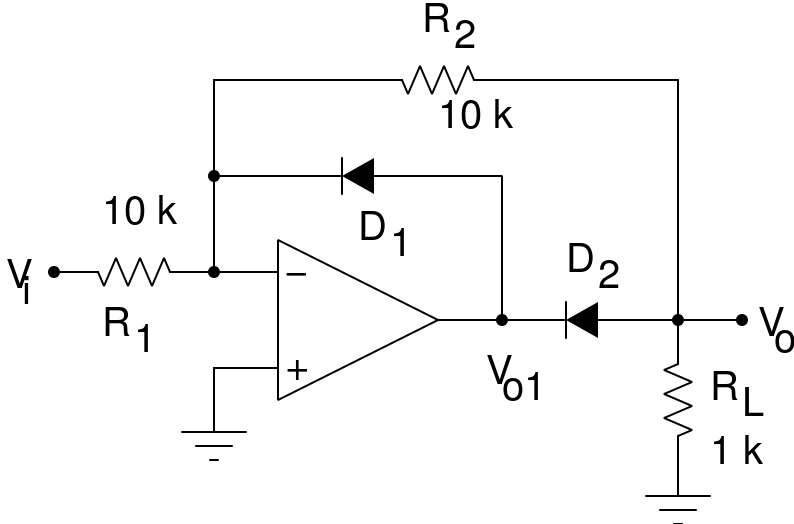
\includegraphics[width = 0.5\linewidth, height = 2.5in]{reports/lab3/half-rect-B.png}
            \caption{Improved half-wave rectifier-B}
        \end{figure}
        \\
        The actual resistance of resistors shown in fig 8 are,
        $R_1 = 9.77\Omegak$, $R_2 = 9.66k\Omega$, $R_L = 0.96k\Omega$.\\
        In this rectifier, the current will flow for $V_i > 0$.
        \\
        
        \textbf{(A) f = 100Hz}\\
        
        The observed waveform of this rectifier is: 
        \begin{figure}[H]
            \centering
            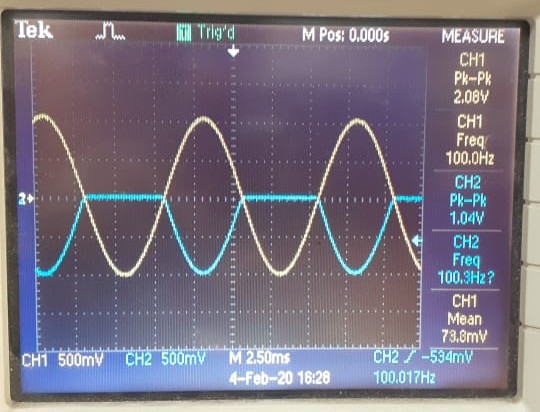
\includegraphics[width = 0.6\linewidth, height = 2.5in]{reports/lab3/half-wave-rect-B-100k.jpeg}
            \caption{Waveform of Improved half-wave rectifier-B}
        \end{figure}
        \\
        $V_o$ vs $V_i$ relationship is given by
        \begin{equation}
            V_o = -\frac{R_2}{R_1} V_i
        \end{equation}
        \begin{figure}[H]
            \centering
            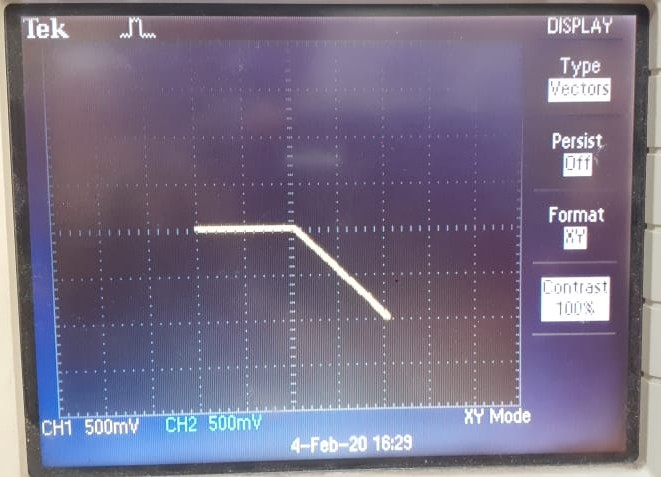
\includegraphics[width = 0.6\linewidth, height = 2.5in]{reports/lab3/half-wave-rect-B.jpeg}
            \caption{$V_o$ vs $V_i$ relationship}
        \end{figure}
        \\
        
        \textbf{(B) With $\mathbf{f = 5kHz :}$}\\
    
        The observed waveform of this rectifier is: 
        \begin{figure}[H]
            \centering
            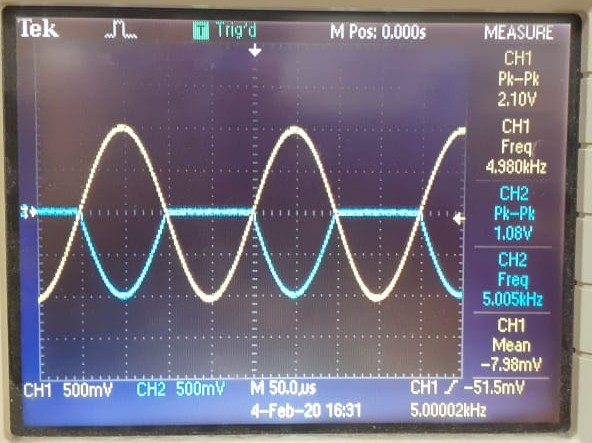
\includegraphics[width = 0.6\linewidth, height = 2.5in]{reports/lab3/half-wave-rect-B-5k.jpeg}
            \caption{Waveform of Improved half-wave rectifier-B}
        \end{figure}
        \\
        Similar, to rectifier-A.\\
        \\
        Here the rectifier conducts for $V_i > 0$. For $V_i < 0$, $V_o$ goes to 0 because at this point the diode D1 conducts and completes the feedback loop not allowing the op-amp to go in saturation. Therefore distortion in the waveform is absent for higher frequencies.

\subsection{Full-wave precision rectifier}
     \begin{figure}[H]
        \centering
        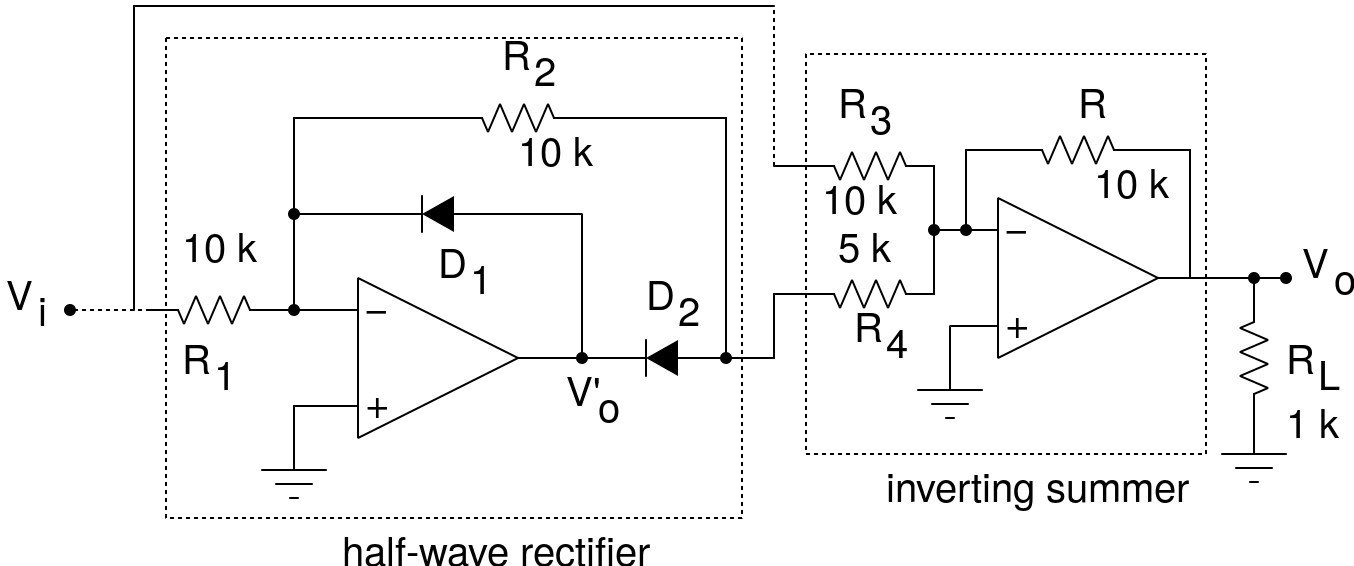
\includegraphics[width = \linewidth, height = 3in]{reports/lab3/full-wave.png}
        \caption{Full-wave precision rectifier}
    \end{figure}   
        The full-wave rectifier is implemented by suitably combining the circuits of half-wave precision rectifier-B and of an inverting summer.\\
        \\
        The actual resistance of resistors shown in fig 8 are,
        $R_1 = 9.77\Omegak$, $R_2 = 9.66k\Omega$, $R_2 = 9.66k\Omega$, $R_3 = 9.88k\Omega$, $R_4 = 5.03k\Omega$, $R_L = 0.96k\Omega$.\\
        \\
        
        \textbf{(A) f = 100Hz}\\
        
        The observed waveform of this rectifier at different frequencies are: 
        \begin{figure}[H]
            \centering
            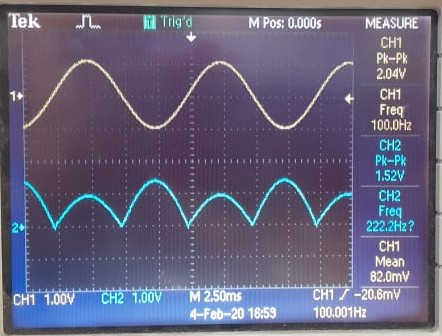
\includegraphics[width = 0.5\linewidth, height = 2in]{reports/lab3/full_wave.jpeg}
            \caption{Waveform of Full-wave precision rectifier for f = 100Hz}
        \end{figure}
        \begin{figure}[H]
            \centering
            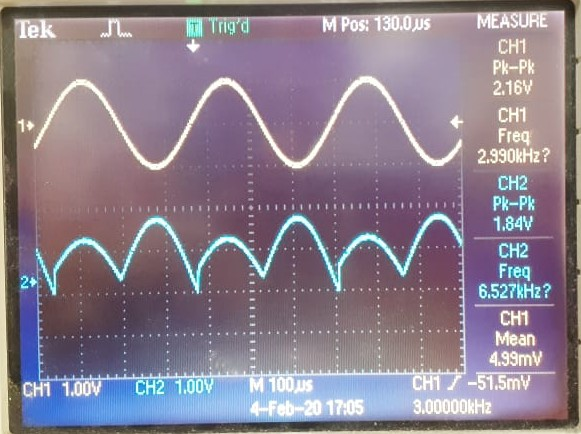
\includegraphics[width = 0.5\linewidth, height = 2in]{reports/lab3/full_wave-3k.jpeg}
            \caption{Waveform of Full-wave precision rectifier for f = 3kHz}
        \end{figure}
        \begin{figure}[H]
            \centering
            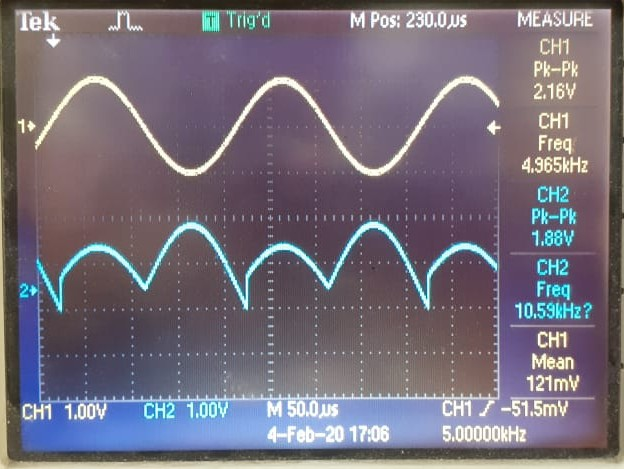
\includegraphics[width = 0.5\linewidth, height = 2in]{reports/lab3/full_wave-5k.jpeg}
            \caption{Waveform of Full-wave precision rectifier for f = 5kHz}
        \end{figure}
        \\
        $V_o$ vs $V_i$ relationship is given by
        \begin{equation}
            V_o = -(\frac{R}{R_3}V_i + \frac{R}{R_4}V_{o1})
        \end{equation}
        \begin{figure}[H]
            \centering
            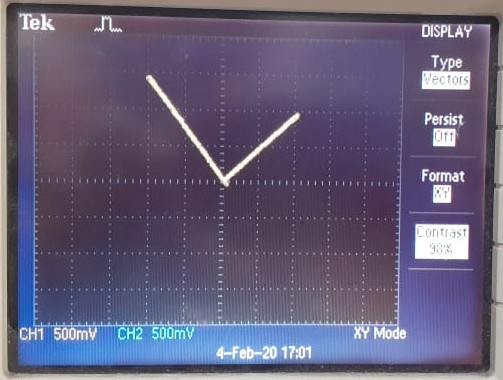
\includegraphics[width = 0.5\linewidth, height = 2in]{reports/lab3/full_wave-xy.jpeg}
            \caption{$V_o$ vs $V_i$ relationship}
        \end{figure}
        \\
        Ideally, $R_3$ and $R_4$ are equal to $R$, so the $V_o$ vs $V_i$ relationship comes out to be symmetric along y-axis. Since here the practical values of resistors are not same, we see unequal weightage given to $V_i$ and $V_{o1}$ in the inverting summer.
        \begin{figure}[H]
            \centering
            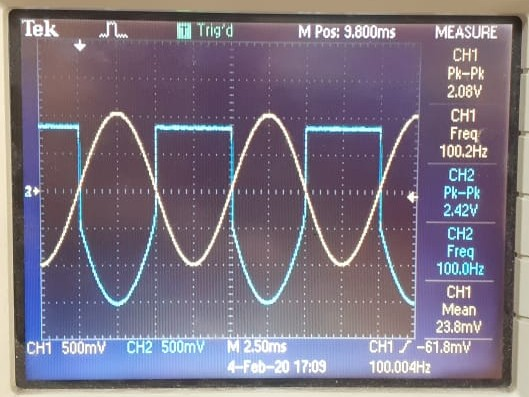
\includegraphics[width = 0.5\linewidth, height = 2in]{reports/lab3/Vo_full.jpeg}
            \caption{waveform of $V'_o$ and $V_i$}
        \end{figure}
        \\
        The full-wave precision rectifier is in saturation region for
        $V_i < 0$ and is in linear region for $V_i > 0$ as is evident from the above figure.
        
\vspace{4cm}

    \begin{thebibliography}{9}

        \bibitem{Analog LAB Manual} 
        Rectifier supporting document 
        \\\texttt{http://wel.ee.iitb.ac.in/teaching\_labs/WEL\%20Site/ee230/Labsheets-2020\\/supporting\_documents/Rectifier\%20circuits.pdf}
        % \bibitem{Datasheet of UA741}
        % Datasheet of OpAmp UA741
        % \\\texttt{https://www.slideshare.net/YongHeuiCho/u-a741}
        
    \end{thebibliography}

\end{document}

